\documentclass[11pt]{article}
\usepackage[margin=3cm]{geometry}
\usepackage[swedish]{babel}
\usepackage[utf8]{inputenc}
\usepackage[T1]{fontenc}
\usepackage{fancyhdr}
\usepackage{ragged2e}
\usepackage{titling}
\usepackage{graphicx}
\usepackage{pbox}
\usepackage{tabularx}
\usepackage{longtable}
\usepackage{tabu}
\usepackage{url}
\usepackage{float}
\usepackage[hidelinks]{hyperref}
\usepackage[backend=biber,style=ieee]{biblatex}
\usepackage{csquotes}

\addbibresource{refs.bib}

\graphicspath{ {images/} }
\newcommand{\subtitle}[1]{%
  \posttitle{%
    \par\end{center}
    \begin{center}\large#1\end{center}
    \vskip0.5em}%
}


\newcounter{refc}
\setcounter{refc}{1}
\newcommand{\reff}{
	\therefc
	\stepcounter{refc}
}

\pagestyle{fancy}


\date{}
\pagenumbering{roman}
\chead{Sensorer till autonom robot}
\rhead{\today}
\lhead{}
\lfoot{
	TSEA56 
	\\
	ISY
}
\rfoot{
	Andreas Brorsson, \textit{andbr981}
	\\
	Nikolaj Agafonov, \textit{nikag669}
}

\begin{document}
\begin{titlepage}
\begin{center}
TSEA56 - Kandidatprojekt i elektronik \\[0.5in]
{\Large\bfseries Sensorer till autonom robot }\\
%
\vspace{4\baselineskip}
%
Version 1.0\\
\vspace{2\baselineskip}
%
Agafonov, Nikolaj, 
\texttt{nikag669}
\\
Brorsson, Andreas, 
\texttt{andbr981}
\\


\vspace{2\baselineskip}
\today

\vspace{23\baselineskip}
Status
\begin{table}[b]
\centering
\begin{tabular}{|l|l|l|} \hline
 Granskad & -- & datum  \\ \hline
 Godkänd  & -- & datum \\ \hline 
\end{tabular}
\end{table}

\end{center}
\end{titlepage}

\pagebreak
\begin{center}

\section*{PROJEKTIDENTITET}
2015/VT, Undsättningsrobot Gr. 2
\\
Tekniska högskolan vid Linköpings Universitet, ISY
\\[0.5in]
\begin{table}[h]
\begin{tabular}{|l|p{0.3\linewidth}|l|l|} \hline
Namn & Ansvar & Telefon & E-post \\[0.1in] \hline
Nikolaj Agafonov & Dokumentansvarig (DA) & 072-276 99 46 & nikag669@student.liu.se \\ \hline
Adnan Berberovic & Projektledare (PL) & 070-491 96 07 & adnbe196@student.liu.se \\ \hline
Andreas Brorsson & Testansvarig (TA) & 073-524 44 60 & andbr981@student.liu.se \\ \hline
Fredrik Fridborn & Designansvarig Sensormodul (DSE) & 073-585 52 01 & frefr166@student.liu.se \\ \hline
Robert Oprea & Designansvarig Styrmodul (DST) & 070-022 10 18 & robop806@student.liu.se \\ \hline
Måns Skytt & Designansvarig Kommunikationsenhet (DK) & 070-354 28 84 & mansk700@student.liu.se \\ \hline
\end{tabular}
\end{table}


E-postlista för hela gruppen: adnbe196@student.liu.se
\\[1in]
Kund: Kent Palmkvist, 581 83 Linköping,
Kundtelefon: 013-28 13 47, kentp@isy.liu.se
\\[1in]

Kursansvarig: Tomas Svensson, 013-28 13 68, tomass@isy.liu.se
\\
Handledare: Olov Andersson, 013-28 26 58, Olov.Andersson@liu.se
\end{center}
\pagebreak

\tableofcontents

\pagebreak

\section*{Dokumenthistorik}
\begin{table}[h]
\begin{tabular}{|l|l|l|l|l|} \hline

Version & Datum & Utförda förändringar & Utförda av & Granskad \\[0.1in] \hline
0.1 & 2015-03-05 & Första utkastet & NA, ABr & - \\ \hline
1.0 & 2015-04-01 & Slutlig version & NA, ABr & - \\ \hline


\end{tabular}
\end{table}


\pagebreak

\pagenumbering{arabic}

\begin{flushleft}

%% -------------------------------------- ////////// ---------------------

\section{Inledning}
Denna förstudie om sensorer tar upp frågeställningar som uppkommer när en autonom robot ska konstrueras. Vilka sensorer som passar till en undsättningsrobot och hur dessa fungerar. Denna rapport behandlar de sensorer som finns tillgängliga i kursen TSEA56 och är lämpliga att använda på en undsättningsrobot. En jämförelse mellan sensorer som utför samma uppgift ställs mot varandra och vilka sensorer är nödvändiga på roboten. 
 
\subsection{Introduktion till Sensorer}
En sensor är en anordning för att konvertera en form av energi till en annan form. Energin kan vara elektromagnetisk, mekanisk eller akustisk som konverterars till t.ex. en spänning. En dator behöver digital data för att kunna göra beräkningar, därför transformeras spänningen från sensorn via en A/D-omvandlare till digital data som kan processeras. 
\\[0.1in]
Sensorer som den autonoma undsättningsroboten behöver är:
\begin{itemize}
\item Avståndssensorer för att mäta avståndet till väggar och hinder.

\item Reflexsensor eller RFID-avläsare för att ta reda på när roboten kommit fram till målet.

\item Gyro, för att beräkna hur mycket roboten har roterat vid svängar eller rotation.

\end{itemize}

\subsection{Syfte}

Syftet med förstudien är att ge en bred kunskapsbas om sensorer för att kunna jämföra sensorer och komma fram till vilka sensorer som passar bäst till en undsättningsrobot i kursen TSEA56.

\subsection{Mål}
Målet med förstudien är:
\begin{itemize}

\item Att beskriva och analysera ovannämnda sensorer.

\item Att få en fördjupning i ämnet och en bred kunskapsbas av sensorer.

\item Att jämföra ovannämnda sensorer och deras fördelar och nackdelar.

\item Att med hänsyn till jämförelsen rekommendera (bestämma) vilka sensorer som bör användas i byggandet av en undsättningsrobot i kursen TSEA56.

\end{itemize} 


\subsection{Parter}
Utöver de personer som är redogjorda för i projektidentiteten är följande personer delaktiga i förstudien.
\begin{itemize}
\item Kent Palmkvist - Beställare
\item Kristoffer Öfjäll - ISY-handledare
\item Birgitte Saxstrup - TEMA-handledare
\end{itemize}

\subsection{Begränsningar}
Det är bara de sensorer som finns tillgängliga i kursen TSEA56 som kommer att undersökas. Eftersom förstudien skrivas på begränsad tid kommer bara de mest relevanta sensorer att undersökas. Vilka sensorer som finns tillgängliga i kursen specificeras på Vanheden \autocite{vanheden}. Vanheden är en webbplats där ISY har samlat datablad och annan nyttig information till de praktiska delarna i kursen.


%% -------------------------------------- ////////// ---------------------

\section{Problemformulering}
I förstudien ska sensorer som finns tillgängliga för att bygga en autonom undsättningsrobot i kursen TSEA56 beskrivas. Det finns olika sensorer att tillgå och sensorer som utför samma uppgift. Uppgiften är att ta reda på vilka sensorer som behövs till roboten för att den ska kunna utföra sitt uppdrag.
\\[0.1in]
Därav är det viktigt att beskriva varje sensor utförligt och presentera fakta för varje sensor för att kunna utvärdera vilka som är lämpliga att använda. Nedstående frågor används som underlag: 
\\[0.1in]

\begin{itemize}

\item Hur fungerar sensorn?

\item Vilka fysikaliska principer används?

\item Vad har sensorn för prestanda?

\item Är sensorn känslig för någon störning?

\end{itemize}


När dessa frågor är besvarade för varje sensor jämförs de. Jämförelsen ger resultatet som sammanfattar vilka och hur många sensorer som bör användas på undsättningsroboten samt var på roboten bör de monteras.


 \subsection{Metod}
För att besvara frågeställningarna kommer forskning bedrivas genom litteraturgranskning. Vilka sensorer som ska granskas begränsas av de som finns på Vanheden där tillgång till datablad även finns. För ytterligare information om hur sensorerna fungerar kommer vetenskapliga artiklar att användas. Data ska sammanställas och presenteras för att sedan analyseras för att få fram ett resultat.

\section{Labyrint}
Undsättningsroboten har för uppgift att utforska en labyrint med en area på högst 6x6m. Roboten ska kunna reglera sig själv när den befinner sig i det autonoma läget, d.v.s. att roboten ska korrigera sin riktning på så sätt att avståndet mellan labyrintens väggarna till roboten blir samma. Korridorer i labyrinten ska vara 0.4m breda och alla hörn får utgöras av vinkelräta väggelement därmed bör roboten vara utrustad med lämpliga sensorer. Mål och startposition i labyrinten skall vara 40x40cm och markeras med en svart tejp på marken.

\section{Motivation till valet av sensorer}
Avståndssensorer bör finnas på alla sidor om roboten för att känna av väggar och hinder. Det är även praktiskt att ha fler sensorer på vissa sidor t.ex. på robotens höger och vänstersida. Detta behövs för att kunna reglera robotens riktning och hålla den centrerad, så att roboten skulle kunna köra utan att slingra sig fram. Dessutom kan det behövas sensorer av olika detektionsområden på robotens sidor för att kunna samla så mycket data som möjligt, till exempel för att rita karta över labyrinten på ett effektivt sätt. 
\\[0.1in]

För att avgöra robotens vridning och därmed undvika att roboten fastnar vid svängar behöver en vinkelhastighetssensorn kopplas till roboten. Eftersom korridorerna i labyrinten där roboten ska köra är begränsade är det lämpligt att använda sensorer som har relativt lågt detektionsområde. 
\\[0.1in]

Detektionsområdets undre gränsen är viktigt för mätnoggrannhet vid små avstånd för att roboten inte ska kollidera. Ju lägre denna gränsen är desto närmare till väggen kan roboten röra sig.  Roboten måste även ha en sensor som kan detektera startposition och mål. För dessa syften kan antingen en reflexsensor eller en RFID-avläsare användas.
\\[0.1in]


\section{Avståndsmätare}
Roboten kommer att vara utrustad med aktiva avståndsmätare, vilket betyder att de sensorerna kommer att skicka ut vågor kontinuerligt under den autonoma styrningen. En avståndssensor skickar ut antingen en serie akustiska eller elektromagnetiska pulser som reflekteras tillbaka från objekt som pulserna träffat. Sensorn registrerar när pulserna kommer tillbaka eller reflektionsvinkel för att beräkna avståndet till objektet. Optiska och akustiska sensorer är begränsade med olika avståndsintervall som sensorer kan beräkna avstånd på.
 
\subsection{Optisk avståndsmätare}
Det finns olika typer av optiska sensorer. Generellt finns det en sändare och en mottagare. Dessa kan antingen finnas i en och samma enhet eller separat. Principen bygger på att skicka ut en ljusstråle och detektera den efter att den har reflekterats från ett objekt, till vilken avståndet mäts \autocite{Fotoceller}.

\pagebreak

\subsubsection{Fysikaliska principer} 
För att mäta avståndet till objekt används trianguleringsprincipen. Detta medför att avståndet som sensorn beräknat fram beror på det reflekterade ljusets vinkel. Se figur~\ref{fig:reflect} nedan. Det finns tre typer av funktionaliteten som väljs beroende på omgivningen. Den kan vara bakgrundsavbländande, förgrundsavbländande eller med fixerat fokus. I det första fallet detekteras inte objekt som är längre bort än avkänningsområdet, i det andra detekteras objekt inte om det finns närmare än avkänningsområdet och i det sista fallet detekteras objekt bara om de befinner sig i avkänningsområdet \autocite{Fotoceller}.

\begin{figure}[h]
\centering
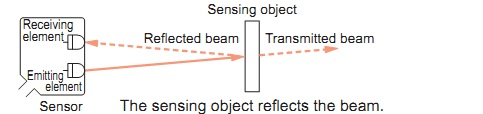
\includegraphics[scale=1]{reflect}
\caption{Direktavkänning - ljuset reflekteras från objektet \autocite{Fotoceller}.}
\label{fig:reflect}
\end{figure}

\subsubsection{Data och signaler}
Direktavkännande sensorer med fixerat fokus kommer att användas i robotens konstruktion. Efter att en sensor har mätt avståndet till en vägg eller något annat objekt, konverteras resultatet till respektive spänningsvärde och sedan skickas ut av sensorn. Data behandlas vidare av en A/D-omvandlare för att kunna behandlas i processorn \autocite{Fotoceller}, \autocite{diagram1}.

\subsubsection{Prestanda}
De optiska sensorer som finns till förfogande visar ett mönster av att antingen kunna läsa avstånd på från relativt kort avstånd till relativt kort avstånd. Eller så kan de mäta från ett relativt långt minsta avstånd till relativt långt maximalt avstånd t.ex. 4-30 cm och 20-150 cm. 
\\[0.1in]
Detta beror på att dessa sensorer egentligen kan detektera kortare avstånd än vad som är angivet som det minsta avståndet i databladen, och de angivna avståndsintervall i databladen anger endast sensorernas maximala avläsningsavstånd. Sensorernas mätningar kan resultera i samma spänningsvärde för två olika avstånd.

\pagebreak

I figur~\ref{fig:diagram} nedan erhålls ett maximum i ut-spänning vid avståndet 5 cm(syns på x-axeln), detta är vad sensorn kommer att ange som sitt minimi-avstånd i dess datablad. För avstånd både mindre och större än 5cm visas samma utspänning, som t.ex för 2.5 volt ges både 4 och 9 cm. Därför programmeras roboten till att alltid tolka signalerna från minsta-avstånd (maximi-punkten) till största avstånd, angivet i databladet \autocite{diagram1}.
\\[0.1in]

\begin{figure}[H]
\centering
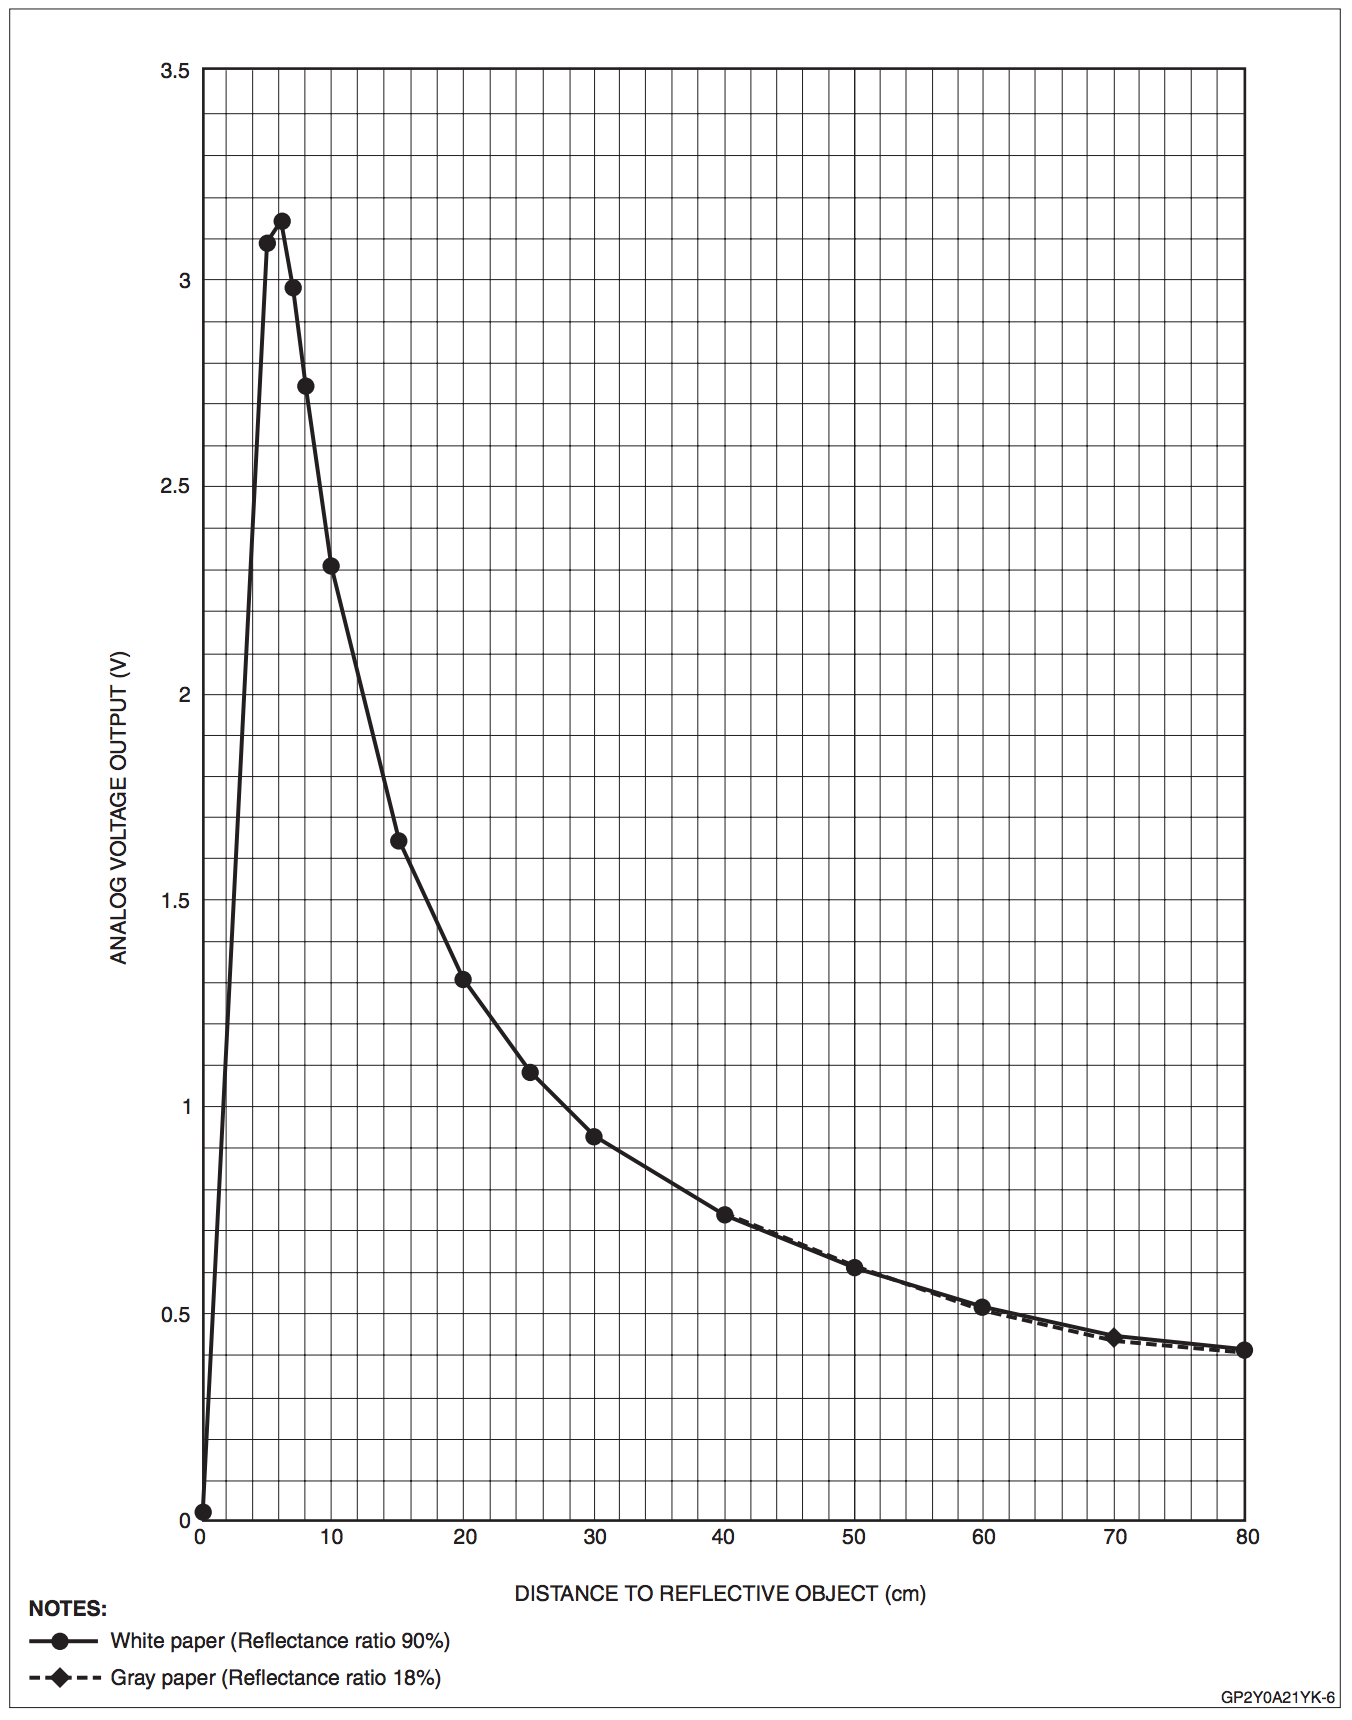
\includegraphics[scale=0.28]{diagram}
\caption{Diagram på utsignal mot avstånd \autocite{diagram1}.}
\label{fig:diagram}
\end{figure}

För optiska avståndsmätare som är tillgängliga, fås utsignalen i form av ett spänningsvärde. Detta värdet fås cirka 16ms eller 38ms efter en mätning påbörjas, beroende på sensorn.

\subsubsection{Störkänslighet}
De optiska avståndsmätarna jobbar i det infraröda spektrummet, detektorn kan då bli störd av solljus och miljöer med starkt omgivande ljus eller reflektioner. Om objekt eller hinder är genomskinligt eller har en starkt reflekterande yta kan mätningen bli störd eller inte fungera alls.    

 \subsection{Akustisk avståndsmätare}
 Akustiska sensorer registrerar ljud med en mikrofon. Sensorn kan bestämma både våglängd och intensitet på det registrerade ljudet. Med kunskap om utbredningshastigheten för ljudvågor kan även avståndet till ett objekt beräknas \autocite{spridning}.
\\[0.1in]
 
För akustiska avståndsmätare skickar och mottager mätaren ultraljud. Fördelen med ultraljud är att människan inte kan höra det, för att frekvensen ligger över 20kHz. Ultraljud används även för att minska störning från omgivning då det sällan förekommer naturligt. Om avståndsmäting sker under vatten kallas det sonar.      
 
\subsubsection{Fysikalisk princip}
Principen för avståndsmätning med ultraljud är att en högtalare skickar ut ett antal pulser med ultraljud. Ljudet träffar något objekt som reflekterar tillbaka ljudet som registreras av mikrofonen på avståndsmätaren. Men kunskap om ljudets hastighet och tiden det tar för ljudet att komma tillbaka går det att beräkna avståndet till objektet.
\\[0.1in]

\begin{figure}[H]
\centering
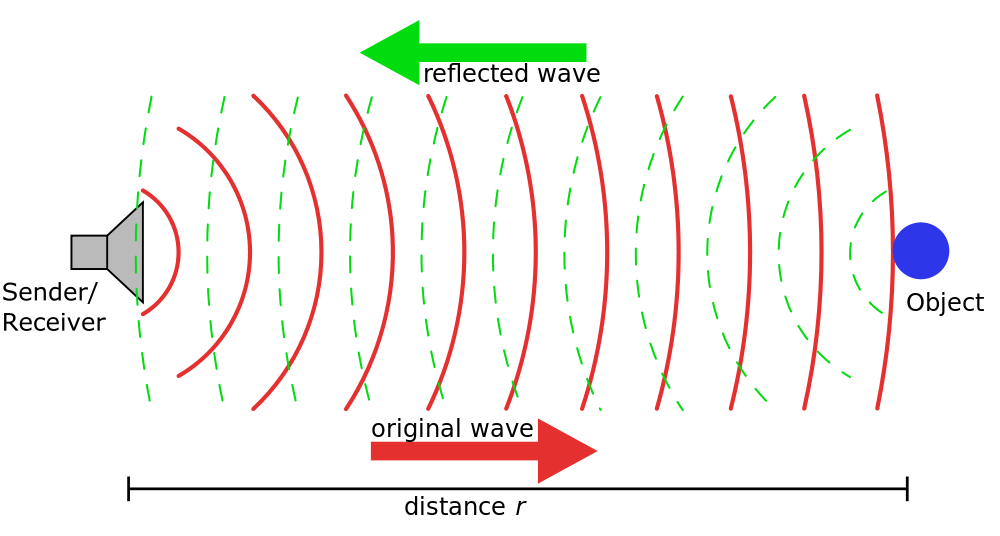
\includegraphics[scale=0.32]{sonar}
\caption{Hur avståndsmätning med ultraljud fungerar \autocite{sonar}.}
\label{fig:sonar}
\end{figure}

\subsubsection{Data och signaler}
Ultraljudssensorn skickar en puls, som är ungefär från 100us till 18ms lång, till en processor, där avståndet till ett objekt beräknas med avseende på pulsens bredd. Om ljudet inte når fram till något objekt, kommer processorn att ta emot en puls som är cirka 36ms lång.
 
\subsubsection{Prestanda}
Den ultraljudssensorn som finns till förfogande kan mäta avstånd från 3cm till 3m. Fördelen med sensorn är att dess mätdata är oberoende föremålets förmåga att reflektera eller absorbera ljus.  

\pagebreak 
 
 \subsubsection{Störkänslighet}
När en ultraljudsensor skickar ut pulserna, sprids ljudet ut radiellt från sändaren. Detta resulterar i att det detekterade ljudet inkommer från vissa infallsvinklar som ligger innanför ett konformat spektrum se figur~\ref{fig:ultra} nedan. Roboten som antar att mätningar sker ortogonalt från sändaren kan få felaktiga mätvärden. 

\begin{figure}[H]
\centering
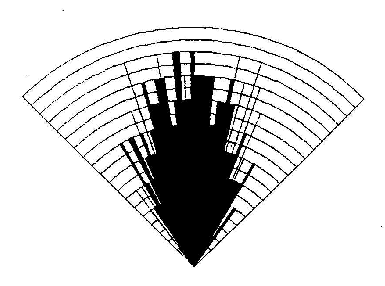
\includegraphics[scale=0.7]{ultra}
\caption{Spridning i ultraljudsavståndsmätarens mätningar \autocite{spridning}. }
\label{fig:ultra}
\end{figure}


 \section{Vinkelhastighetssensor}
 Vinkelhastighetsmätare som ofta refereras till som gyroskop är en mekanisk sensor som kan detektera förändringar i vinkelhastighet. Denna sortens sensorer kan användas för att komplettera data, som en processor kan använda för att räkna ut hur mycket roboten har roterat eller hur långt en sväng är gången. Utan gyrot, kan processorns beräkningar inte litas på 100\% för att hjulen kan glida på underlaget eller slira. Detta skulle resultera i att roboten tror den har förflyttat sig när den stått still eller förflyttat sig för lite mot vad den beräknat.
 
\pagebreak 
 
 \subsection{Fysikalisk princip}
Gyrot känner av vinkelhastigheten när sensorn roterar horisontellt kring Z-axeln, se figur~\ref{fig:gyro} nedan. MLX90609 har en mekanisk struktur som oscillerar då Corioliskraften verkar på den. Denna kraft uppstår endast om modulen är i rörelse. Mekaniska vibrationer som skapas registreras och transformeras sedan till utspänningen \autocite{vanheden-gyro}.
 
\begin{figure}[H]
\centering
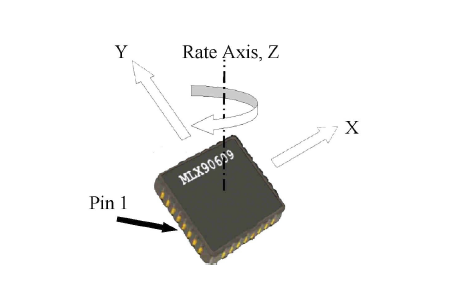
\includegraphics[scale=0.6]{gyro}
\caption{Vinkelhastighetssensor MLX90609 med axlar \autocite{vanheden-gyro}.}
\label{fig:gyro}
\end{figure}
 
\subsection{Data och signaler}
Gyrot beräknar spänningen som beror på robotens vinkelhastighet med avseende på omgivningen. Efter detta konverteras spänningen med en intern A/D-omvandlare till ett digitalt värde. När gyrot har mottagit en operations-kod (bestående av 8 eller 16 bitars ord) från styrmodulen skickas svaret till styrmodulen via en SPI-buss. Data (16 bitars ord) som styrmodulen får från VHS behöver sedan omvandlas till ett respektive värde på vinkelhastiget mätt i grader per sekund. 
  
\subsection{Prestanda}
Gyrot kan läsa av vinkelhastighet upp till 300 grader/s. Gyrot är en enskild modul som kopplas direkt till master-modulen. Det betyder att gyrot inte behöver kopplas till en modul som behöver göra extra beräkningar. A/D-omvandlingen tar cirka 90 mikrosekunder att utföra och det tar 24 klockcykler för gyrot att ta emot ett meddelande från master-modulen och skicka tillbaka ett svar.

 \subsection{Störkänslighet}
För att mäta robotens vinkelhastighet med MLX90609 ska modulen vara placerad vinkelrätt mot rotationsaxeln. Sensorn är känslig för lutning och hinder vilket resulterar i avvikelser från robotens riktiga vinkelhastighet.

\pagebreak 
 
\section{Reflexsensor}
Reflekssensorn är sensor som skickar ut ljus och sedan mäter styrkan i det reflekterade ljuset. Reflekssensorn består av en lysdiod som sänder ut infrarött ljus och en fototransistor som detekterar infrarött ljus.

 \subsection{Fysikalisk princip}
Reflexsensors ljusdiod som radierar infrarött ljus är tänd hela tiden. När fototransistorn blir exponerad för infrarött ljus släpper transistorn igenom ström vilket gör att utgången blir låg. När mindre ljus reflekteras som t.ex. när en svart tejpbit sitter i vägen släpper transistorn igenom mindre ström och utgången blir hög \autocite{vanheden_reflex}. 

\begin{figure}[H]
\centering
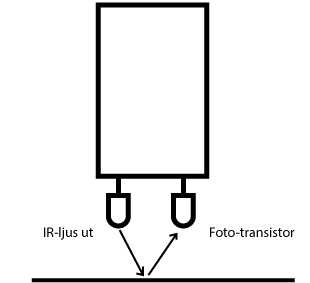
\includegraphics[scale=0.5]{Reflexsensor}
\caption{Hur en reflexsensor fungerar.}
\label{fig:reflex}
\end{figure}
 
\subsection{Data och signaler}
Även om tanken är att konstruktionen ska ge en diskret hög och låg signal så är inte fallet så. Utsignalen måste gå genom en A/D-omvandlare och tester måste genomföras för att bestämma när sensorn anses gå hög.
 
\subsection{Prestanda}
Sensorn placeras några millimeter från mätytan och skickar ut analog data.

\subsection{Störkänslighet}
Fotoresistorn är känslig för infrarött ljus, väldigt starka ljuskällor med infraröttljus i rummet skulle kunna störa sensorn. Avståndet mellan sensorn och ytan ska vara ett par millimeter, därför att om sensorn sätts för långt ifrån ytan kan det reflekterade infraröda ljuset bli för svagt och sensorn går hög felaktigt. Det måste vara tydlig kontrast mellan yta och markering.

\pagebreak
 
\section{RFID}
Tekniken RFID är ett akronym för 'radio frequency identification' och är en teknik som har två huvudkomponenter, en avläsare och en tagg. Där avläsaren skickar ut en radiosignal till en tagg som skickar tillbaka information till avläsaren.
\\[0.1in]

RFID-tekniken har likheter med den föråldrade tekniken med en optisk avläsare som läser stäckkod för att få fram ett ID-nummer. På samma sätt fungerar RFID men eftersom tekniken använder sig av radiovågor istället för optisk avläsning behöver inte avläsaren optiskt se taggen. En annan fördel är att en tagg kan bära på mer information än bara ett ID, de billigaste brukar stega in med ett minne på 2 KB \autocite{rfid1}, \autocite{rfid_faq}.    
\\[0.1in]

Avståndet mellan en avläsare och en tagg kan variera från några centimeter till flera hundra meter beroende på vilken sort tagg som används. Det finns tre olika sorter, passiv, semipassiv och aktiv. Aktiv och semipassiv har strömkällor inkopplade och kan skicka mer data och över längre avstånd, jämfört med en passiv tagg som blir strömförsörjd av radiosignalen från avläsaren \autocite{Weis_rfid}. 
\\[0.1in]

 \subsection{Fysikalisk princip}
En avläsare skickar ut radiovågor i 120-140 kHz området. En passiv tagg som upptäcktes av en avläsare blir strömförsörjd genom induktion som ger den kraft att skicka tillbaka data som sparats på taggen. Resultatet av att passiva taggen använder induktion för att bli strömförsörjd är att avståndet när data ska överföras mellan tagg och avläsare blir kort, ungefär mellan 10-20cm. Semipassiva och aktiva taggar kan därför skicka data över längre avstånd med batteri eller aktiv försörjning.  

\subsection{Data och signaler}
Avläsaren skannar kontinuerligt efter en tagg och skickar data seriellt till mikroprocessorn. När en tagg hittats jämförs data med innehållet i ett register i mikroprocessorn \autocite{vanheden_rfid}. 
 
\subsection{Prestanda}
Läsavståndet mellan avläsaren och taggen är upp till 10cm, avläsaren behöver inte se taggen utan bara vara inom avståndet. Olika taggar kan ge olika information som avläsaren kan programmeras efter. Taggar kan placeras i många olika miljöer och fungerar nära metall, vätskor och smuts.  
 
\subsection{Störkänslighet}
Om flera taggar skickar tillbaka data samtidigt till avläsaren kan avläsaren få svårt att veta att det är mer än en tagg som skickar data och även blanda ihop data. Den passiva taggen som finns tillgänglig är avståndsberoende och det finns en liten chans att roboten skulle kunna missa taggen. Om taggen är på gränsen kan avläsningen bli fel. Vart taggen är placerad relativt mot avläsaren påverkar hur långt avstånd avläsaren kan hitta en tagg.


\section{Resultat och slutsatser}
Genom att jämföra olika sensorer bestämdes vilka sensorer som är lämpliga för robotens konstruktion. Först bedömdes robotens begränsningar, syfte och användningsområde och därmed kunde minsta antalet sensorer bestämmas och deras typer i syfte att roboten skulle kunna uppnå uppställda mål. 
\\[0.1in]

Eftersom antalet sensorer som kan kopplas till varje virkort är begransat valdes sensorer som är nödvändiga för att roboten skulle klara av alla uppställda krav. De sensorer som kommer att användas är:

\begin{itemize}
\item 5 st optiska avståndsmätare GP2Y0A41SK (4-30 cm).
\item 2 st optiska avståndsmätare GP2Y0A21 (10-80 cm).
\item En reflexsensor.
\item En vinkelhastighetssensor.
\end{itemize}

En avståndssensor på robotens framsida för att mäta korta avstånd och inte köra på objekt. Två sensorer som mäter korta avstånd på varje sida för att kunna beräkna robotens vinkel och position mellan väggarna. Samt en avståndssensor för långa avstånd på mitten av vardera sida för att ge information om objekt på längre avstånd. Data från dessa sensorer ska användas i PD-regleringen och utritandet av labyrintens karta.
\\[0.1in]

Vinkelhastighetssensorn behövs för att kontrollera hastigheten av robotens vridning och därmed kunna optimera autonom styrning vid kurvor och rotation. Roboten ska ha en sensor som kan identifiera målet. Detta åstadkommer reflexsensor, som fästas på robotens undersida.


\subsection{Diskussion}
En av de stora skillnaderna mellan akustisk och optisk avståndssensor är detektionsområdets vinkel. För akustisk mottagare är detektionsområdet 30 grader brett medans optiska mottagarens detektionsområde är cirka 6 grader. Vilket säger att den optiska sensorn kommer ge mer noggran data.
\\[0.1in]

Enligt databladet är den akustiska sensormodulen ganska stor och duger inte för relativt små robotar. Dessutom är akustiska sensorer avsedda för att mäta avståndet från 3 cm till 3 m och roboten har inget behov av att mäta relativt stora avstånd. Fördelen med både optisk och akustisk avståndsmätare är att människan inte kan uppfatta vågorna som skickas ut, den optiska sensorn använder infrarött ljus och akustiska sensorn använder ultraljud.
\\[0.1in]

En fråga som dyker upp är om vinkelhastighetssensorn är absolut nödvändig eller inte. Roboten kan tänkas klara vissa av sina uppgifter med hjälp av endast avståndssensorer. Dock kan avståndssensorerna vara missvisande eller svårtolkade under en rotation och robotens egna uträkning om hur långt en rotation är gången blir fel om däcken slirar eller glider. Gyrot beräknar rotationen och ger korrekt data så att en rotation blir effektiv utan att felkorrigering behövs.
\\[0.1in]

Orsaken till att reflexsensorn har valts och inte RFID-avläsaren är framför allt att roboten inte ska känna av olika mål (det finns bara ett). Jämfört med reflexsensorn har RFID-avläsaren större komplexitet och kan hantera olika taggar. Detta behövs inte för autonom styrningen av en kartläggningsrobot i kursen TSEA56. Reflexsensorn är enkel darför att den skickar ut en signal som antingen blir hög eller låg beroende om målet hittats eller inte.
\\[0.1in]

Däremot skulle RFID-avläsaren kunna vara säkrare än reflexsensorn med avseende på störkänslighet. De reflekterade ljusets intensitet från reflekssensorn avtar snabbt när avståndet mellan sensor och mark ökar, därmed kan sensormodulen missuppfatta signalen. Detta måste tas hänsyn till vid uppbyggandet av roboten och reflexsensorn bör placeras så nära marken som möjligt.



\setcounter{secnumdepth}{0}
\pagebreak


\printbibliography


\setcounter{secnumdepth}{2}
\end{flushleft}

\end{document}
